%%%%%%%%%%%%%%%%%%%%%%%%%%%%%%%%%%%%%%%%%
% Masters/Doctoral Thesis 
% LaTeX Template
% Version 1.43 (17/5/14)
%
% This template has been downloaded from:
% http://www.LaTeXTemplates.com
%
% Original authors:
% Steven Gunn 
% http://users.ecs.soton.ac.uk/srg/softwaretools/document/templates/
% and
% Sunil Patel
% http://www.sunilpatel.co.uk/thesis-template/
%
% License:
% CC BY-NC-SA 3.0 (http://creativecommons.org/licenses/by-nc-sa/3.0/)
%
% Note:
% Make sure to edit document variables in the Thesis.cls file
%
%%%%%%%%%%%%%%%%%%%%%%%%%%%%%%%%%%%%%%%%%

%----------------------------------------------------------------------------------------
%	PACKAGES AND OTHER DOCUMENT CONFIGURATIONS
%----------------------------------------------------------------------------------------

\documentclass[11pt, oneside]{Thesis} % The default font size and one-sided printing (no margin offsets)

\graphicspath{{Pictures/}} % Specifies the directory where pictures are stored

\usepackage[square, numbers, comma, sort&compress]{natbib} % Use the natbib reference package - read up on this to edit the reference style; if you want text (e.g. Smith et al., 2012) for the in-text references (instead of numbers), remove 'numbers' 
\usepackage{alltt}
\usepackage{color}
\title{\ttitle} % Defines the thesis title - don't touch this

% Added by Haavard %---------------------------------------------------------------------
\usepackage[utf8]{inputenc} % Norwegian letters
\usepackage{subcaption}
\usepackage[font={small, it}]{caption} % captions on figures and tables
\usepackage{graphicx}
\usepackage{color}
\usepackage{hyperref} % Use \autoref{ and \nameref{
\hypersetup{backref,
  colorlinks=true,
  breaklinks=true,
  %hidelinks, %uncomment to make links black
  linkcolor=blue,
  urlcolor=blue,
  citecolor=blue
}
\usepackage[all]{hypcap} % Makes hyperref jup to top of pictures and tables
% --------------------------------------------------------------------------------------

% Added by Jorgen, for source code listing %-------------------------------------------
\usepackage{wrapfig}

\usepackage{listings}
\usepackage{xcolor}
\newcommand{\textcolordummy}[2]{#2}

\definecolor{mygray}{rgb}{0.4,0.4,0.4}
%\definecolor{mycyan}{rgb}{0,0.8,0.6}
\definecolor{mygreen1}{rgb}{0.3,0.6,0.3}
\definecolor{mygreen2}{rgb}{0,0.4,0.1}
\definecolor{myorange}{rgb}{1.0,0.4,0}

\lstset{language=C++,
                basicstyle={\color{black}\footnotesize\ttfamily\let\textcolor\textcolordummy},
                %identifierstyle=\color{green},
                keywordstyle={\color{blue}\footnotesize\ttfamily\let\textcolor\textcolordummy},
                %keywordstyle={\color{blue}\footnotesize\ttfamily\let\textcolor\textcolordummy},
                directivestyle={\color{mygreen1}},
                emph={int,char,double,float,unsigned},
                emphstyle={\color{mygreen2}},
                %
                stringstyle={\color{myorange}\footnotesize\ttfamily\let\textcolor\textcolordummy},
                %stringstyle={\color{orange}\footnotesize\ttfamily\let\textcolor\textcolordummy},
                commentstyle={\color{mygray}\footnotesize\ttfamily\let\textcolor\textcolordummy},
                morecomment=[l][\color{magenta}]{\#}
                %
                showspaces=false,  
                showstringspaces=false, 
                showtabs=false,
                extendedchars=true,
                frame=single,  
}
\lstdefinestyle{FormattedNumber}{%
    literate={0}{{\textcolor{red}{0}}}{1}%
             {1}{{\textcolor{red}{1}}}{1}%
             {2}{{\textcolor{red}{2}}}{1}%
             {3}{{\textcolor{red}{3}}}{1}%
             {4}{{\textcolor{red}{4}}}{1}%
             {5}{{\textcolor{red}{5}}}{1}%
             {6}{{\textcolor{red}{6}}}{1}%
             {7}{{\textcolor{red}{7}}}{1}%
             {8}{{\textcolor{red}{8}}}{1}%
             {9}{{\textcolor{red}{9}}}{1}%
             {.0}{{\textcolor{red}{.0}}}{2}% Following is to ensure that only periods
             {.1}{{\textcolor{red}{.1}}}{2}% followed by a digit are changed.
             {.2}{{\textcolor{red}{.2}}}{2}%
             {.3}{{\textcolor{red}{.3}}}{2}%
             {.4}{{\textcolor{red}{.4}}}{2}%
             {.5}{{\textcolor{red}{.5}}}{2}%
             {.6}{{\textcolor{red}{.6}}}{2}%
             {.7}{{\textcolor{red}{.7}}}{2}%
             {.8}{{\textcolor{red}{.8}}}{2}%
             {.9}{{\textcolor{red}{.9}}}{2}%
             ,
   basicstyle=\footnotesize\ttfamily,%  Optional to use this
}

%---------------------------------------------------------------------

\usepackage{lipsum} % Used for inserting dummy 'Lorem ipsum' text into the template

\usepackage{sectsty} % Allows customizing section commands
\allsectionsfont{\centering \normalfont\scshape} % Make all sections centered, the default font and small caps

\usepackage{fancyhdr} % Custom headers and footers
\pagestyle{fancyplain} % Makes all pages in the document conform to the custom headers and footers
\fancyhead{} % No page header - if you want one, create it in the same way as the footers below
\fancyfoot[L]{} % Empty left footer
\fancyfoot[C]{} % Empty center footer
\fancyfoot[R]{\thepage} % Page numbering for right footer
\renewcommand{\headrulewidth}{0pt} % Remove header underlines
\renewcommand{\footrulewidth}{0pt} % Remove footer underlines
\setlength{\headheight}{13.6pt} % Customize the height of the header

%\numberwithin{equation}{section} % Number equations within sections (i.e. 1.1, 1.2, 2.1, 2.2 instead of 1, 2, 3, 4)
%\numberwithin{figure}{section} % Number figures within sections (i.e. 1.1, 1.2, 2.1, 2.2 instead of 1, 2, 3, 4)
%\numberwithin{table}{section} % Number tables within sections (i.e. 1.1, 1.2, 2.1, 2.2 instead of 1, 2, 3, 4)

\setlength\parindent{0pt} % Removes all indentation from paragraphs - comment this line for an assignment with lots of text

\begin{document}

\frontmatter % Use roman page numbering style (i, ii, iii, iv...) for the pre-content pages

\setstretch{1.3} % Line spacing of 1.3

% Define the page headers using the FancyHdr package and set up for one-sided printing
\fancyhead{} % Clears all page headers and footers
\rhead{\thepage} % Sets the right side header to show the page number
\lhead{} % Clears the left side page header

\pagestyle{fancy} % Finally, use the "fancy" page style to implement the FancyHdr headers

\newcommand{\HRule}{\rule{\linewidth}{0.5mm}} % New command to make the lines in the title page

% PDF meta-data
\hypersetup{pdftitle={\ttitle}}
\hypersetup{pdfsubject=\subjectname}
\hypersetup{pdfauthor=\authornames}
\hypersetup{pdfkeywords=\keywordnames}
% ADDED BY MAGNUS 

%----------------------------------------------------------------------------------------
%	TITLE PAGE
%----------------------------------------------------------------------------------------

\begin{titlepage}
\begin{center}

\textsc{\LARGE \univname}\\[1.5cm] % University name
\textsc{\Large Project TMA4500}\\[0.5cm] % Thesis type

\HRule \\[0.4cm] % Horizontal line
{\huge \bfseries \ttitle}\\[0.4cm] % Thesis title
\HRule \\[1.5cm] % Horizontal line
 
\begin{minipage}{0.4\textwidth}
\begin{flushleft} \large
\emph{Author:}\\
\href{http://www.johnsmith.com}{\authornames} % Author name - remove the \href bracket to remove the link
\end{flushleft}
\end{minipage}
\begin{minipage}{0.4\textwidth}
\begin{flushright} \large
\emph{Supervisor:} \\
\href{http://www.jamessmith.com}{\supname} % Supervisor name - remove the \href bracket to remove the link  
\end{flushright}
\end{minipage}\\[3cm]
 
%\large \textit{A thesis submitted in fulfilment of the requirements\\ for the degree of \degreename}\\[0.3cm] % University requirement text
%\textit{in the}\\[0.4cm]
\groupname\\\deptname\\[2cm] % Research group name and department name
 
{\large \today}\\[4cm] % Date
%\includegraphics{Logo} % University/department logo - uncomment to place it
 
\vfill
\end{center}

\end{titlepage}
%%fakesection - Declaration of Authorship
%----------------------------------------------------------------------------------------
%	DECLARATION PAGE
%	Your institution may give you a different text to place here
%----------------------------------------------------------------------------------------
%\Declaration{

%\addtocontents{toc}{\vspace{1em}} % Add a gap in the Contents, for aesthetics

%I, \authornames, declare that this thesis titled, '\ttitle' and the work presented in it are my own. I confirm that:

%\begin{itemize} 
%\item[\tiny{$\blacksquare$}] This work was done wholly or mainly while in candidature for a research degree at this University.
%\item[\tiny{$\blacksquare$}] Where any part of this thesis has previously been submitted for a degree or any other qualification at this University or any other institution, this has been clearly stated.
%\item[\tiny{$\blacksquare$}] Where I have consulted the published work of others, this is always clearly attributed.
%\item[\tiny{$\blacksquare$}] Where I have quoted from the work of others, the source is always given. With the exception of such quotations, this thesis is entirely my own work.
%\item[\tiny{$\blacksquare$}] I have acknowledged all main sources of help.
%\item[\tiny{$\blacksquare$}] Where the thesis is based on work done by myself jointly with others, I have made clear exactly what was done by others and what I have contributed myself.\\
%\end{itemize}
 
%Signed:\\
%\rule[1em]{25em}{0.5pt} % This prints a line for the signature
 
%Date:\\
%\rule[1em]{25em}{0.5pt} % This prints a line to write the date
%}

%\clearpage % Start a new page
%%fakesection - Quotation page
%----------------------------------------------------------------------------------------
%	QUOTATION PAGE
%----------------------------------------------------------------------------------------

%\pagestyle{empty} % No headers or footers for the following pages

%\null\vfill % Add some space to move the quote down the page a bit

%\textit{``Thanks to my solid academic training, today I can write hundreds of words on virtually any topic without possessing a shred of information, which is how I got a good job in journalism."}

%\begin{flushright}
%Dave Barry
%\end{flushright}

%\vfill\vfill\vfill\vfill\vfill\vfill\null % Add some space at the bottom to position the quote just right

%\clearpage % Start a new page

%----------------------------------------------------------------------------------------
%	ABSTRACT PAGE
%----------------------------------------------------------------------------------------
%%fakesection - Abstract
\addtotoc{Abstract} % Add the "Abstract" page entry to the Contents

\abstract{\addtocontents{toc}{\vspace{1em}} % Add a gap in the Contents, for aesthetics
In this project some basic properties of the least squares method is analysed. Both finite element and spectral methods are discussed, and the implementation is mainly performed using spectral basis functions. The problems analysed in this project are diffusion convection reaction PDEs, both linear and non-linear. The results are compared to standard Galerkin method where both error and condition number is considered. The least squares method is also applied to Galerkin methods to gain stability with great results.  
}

\clearpage % Start a new page

%%fakesection - Acknowledgements 
%----------------------------------------------------------------------------------------
%	ACKNOWLEDGEMENTS
%----------------------------------------------------------------------------------------

%\setstretch{1.3} % Reset the line-spacing to 1.3 for body text (if it has changed)

%\acknowledgements{\addtocontents{toc}{\vspace{1em}} % Add a gap in the Contents, for aesthetics

%The acknowledgements and the people to thank go here, don't forget to include your project advisor\ldots
%}
%\clearpage % Start a new page

%%fakesection - List of contents/figs/tables
%----------------------------------------------------------------------------------------
%	LIST OF CONTENTS/FIGURES/TABLES PAGES
%----------------------------------------------------------------------------------------

\pagestyle{fancy} % The page style headers have been "empty" all this time, now use the "fancy" headers as defined before to bring them back

\lhead{\emph{Contents}} % Set the left side page header to "Contents"
\tableofcontents % Write out the Table of Contents

%\lhead{\emph{List of Figures}} % Set the left side page header to "List of Figures"
%\listoffigures % Write out the List of Figures

%\lhead{\emph{List of Tables}} % Set the left side page header to "List of Tables"
%\listoftables % Write out the List of Tables

%%fakesection - Abbreviations
%----------------------------------------------------------------------------------------
%	ABBREVIATIONS
%----------------------------------------------------------------------------------------

%\clearpage % Start a new page

%\setstretch{1.5} % Set the line spacing to 1.5, this makes the following tables easier to read

%\lhead{\emph{Abbreviations}} % Set the left side page header to "Abbreviations"
%\listofsymbols{ll} % Include a list of Abbreviations (a table of two columns)
%{
%\textbf{LAH} & \textbf{L}ist \textbf{A}bbreviations \textbf{H}ere \\
%%\textbf{Acronym} & \textbf{W}hat (it) \textbf{S}tands \textbf{F}or \\
%}

%%fakesection - Constants/Definitions 
%----------------------------------------------------------------------------------------
%	PHYSICAL CONSTANTS/OTHER DEFINITIONS
%----------------------------------------------------------------------------------------

%\clearpage % Start a new page

%\lhead{\emph{Physical Constants}} % Set the left side page header to "Physical Constants"

%\listofconstants{lrcl} % Include a list of Physical Constants (a four column table)
%{
%Speed of Light & $c$ & $=$ & $2.997\ 924\ 58\times10^{8}\ \mbox{ms}^{-\mbox{s}}$ (exact)\\
%% Constant Name & Symbol & = & Constant Value (with units) \\
%}

%%fakesection - Symbols 
%----------------------------------------------------------------------------------------
%	SYMBOLS
%----------------------------------------------------------------------------------------

%\clearpage % Start a new page

%\lhead{\emph{Symbols}} % Set the left side page header to "Symbols"

%\listofnomenclature{lll} % Include a list of Symbols (a three column table)
%{
%$a$ & distance & m \\
%$P$ & power & W (Js$^{-1}$) \\
%% Symbol & Name & Unit \\

%& & \\ % Gap to separate the Roman symbols from the Greek

%$\omega$ & angular frequency & rads$^{-1}$ \\
%% Symbol & Name & Unit \\
%}

%%fakesection - Dedication
%----------------------------------------------------------------------------------------
%	DEDICATION
%----------------------------------------------------------------------------------------

%\setstretch{1.3} % Return the line spacing back to 1.3

%\pagestyle{empty} % Page style needs to be empty for this page

%\dedicatory{For/Dedicated to/To my\ldots} % Dedication text

%\addtocontents{toc}{\vspace{2em}} % Add a gap in the Contents, for aesthetics

%----------------------------------------------------------------------------------------
%	THESIS CONTENT - CHAPTERS
%----------------------------------------------------------------------------------------

%%fakesection - Notation 
%----------------------------------------------------------------------------------------
%	NOTATION
%----------------------------------------------------------------------------------------

\clearpage % Start a new page

\setstretch{1.5} % Set the line spacing to 1.5, this makes the following tables easier to read

\lhead{\emph{Notation}} % Set the left side page header to "Abbreviations"
\listofsymbols{ll} % Include a list of Abbreviations (a table of two columns)
{
\textbf{CONVENTION} & we let subscript $h$ denote the discretized variables \\
%$u$ & Solution of the partial differential equation\\
%$\mathbf{w} = [w_1 \; w_2 ] $ & Negative gradient of $u$ \\
%$\mathbf{u} = [ \mathbf{w} \; u ]^T$ & Solution to the first order transformation \\ 
%$ R_g $ & Lifting function \\
%$\tilde{\mathbf{u}} = \mathbf{u}-R_g $ & Solution to the first order transformation minus the lifting function \\ 
%$\mathbf{b}$ & Two dimensional vector field \\
%$f$ & loading function\\
%$\mathbf{f} = (0,0,f)$ & loading function for the first order transformation\\
%$\mathcal{L} , \mathcal{B} $ & Linear operators \\
%$(\cdot,\cdot)$ & Inner product, when not specified read as $(\cdot,\cdot)_{L_2}$  \\
%$a(\cdot,\cdot)$ & Bilinear form obtained from standard Galerkin approach \\
%$Q(\cdot,\cdot)$ & Bilinear form obtained from the least squares approach \\
%$\mathring{a}(\cdot,\cdot)$ & Bilinear form obtained from the combined GLS-method\\
%$F(\cdot)$ & Linear form obtained from the least squares approach \\
%$\tilde{F}(\cdot)$ & Linear form obtained from the least squares approach including BC's \\
%$\mathring{F}(\cdot)$ & Linear form obtained from the combined GLS-method \\
%\textbf{Linear Algebra} \\
%$A$ & The stiffness matrix \\
%$G$ & The gradient matrix \\
%$R$ & The reaction matrix \\
%$F$ & The vector obtained from the linear functional $F(\cdot)$ \\ 
%$W$ 	& The diagonal matrix with the GLL-weights \\ 
%$L$ 	& The matrix with the derivative of the lagrange functions in each node \\ 
%$\Phi$ & $W\otimes WL$\\ 
%$\Psi$ & $WL\otimes W$\\ 

%\textbf{LAH} & \textbf{L}ist \textbf{A}bbreviations \textbf{H}ere \\
%\textbf{Acronym} & \textbf{W}hat (it) \textbf{S}tands \textbf{F}or \\
}

\mainmatter % Begin numeric (1,2,3...) page numbering

\pagestyle{fancy} % Return the page headers back to the "fancy" style

% Include the chapters of the thesis as separate files from the Chapters folder
% Uncomment the lines as you write the chapters

%\input{Chapters/Chapter1}
% Chapter Template

\chapter{Introduction} % Main chapter title

\label{introduction} % Change X to a consecutive number; for referencing this chapter elsewhere, use \ref{ChapterX}

\lhead{Chapter 1. \emph{Introduction}} % Change X to a consecutive number; this is for the header on each page - perhaps a shortened title

%----------------------------------------------------------------------------------------
%	SECTION 1
%----------------------------------------------------------------------------------------

%The Navier-Stokes equations have been studied for centuries and describes any fluid in motion. Depending on the properties of the fluid 
%and the circumstances of the flow different variants of these equations are studied. This thesis will restrict itself to the numerical 
%solutions of the incompressible N-S equations.  

The physics regarding fluids in motion are described mathematically by the Navier-Stokes (N-S) equations. 
They are a result of the conservation of momentum and mass and are stated in~\eref{eq:NS}.
This thesis is restricted to numerical solutions of the incompressible N-S equations. For a complete 
description of the necessary assumptions and simplifications it is referred to~\cite{White}.  
An important dimensionless quantity is the Reynolds number $Re$, which describes the ratio between 
momentum forces and viscous forces. For large Reynolds numbers the flow becomes turbulent and a 
large range of scales needs to be resolved. A lot of research has been devoted to determine the
amount of energy present at the different scales of motion, and the interaction between them. 
These ideas has led to turbulence modelling which is based on the 
idea that the effect of the smallest turbulent motions can be modelled, while 
the larger motions are resolved by the numerical grid. 
In this thesis both laminar and turbulent flows will be solved numerically, 
and a physically motivated model for the smallest structures will be compared
with a mathematical filter meant to stabilize the flow.
In addition to solving the N-S equations the 
transport of a passive scalar will also be analysed and compared with a set of reference solutions. 
The software applied in this thesis is Nek5000 which is an implementation of the spectral element method initialized in the 80's.
In addition to validate Nek5000 as a software for analyzing gas dispersion the work in this thesis 
also attempts to make Nek5000 more applicable to cases consisting of more complex geometry. 

This thesis is divided in 3 parts. The first part which consists of the two following chapters are devoted to the physical understanding 
of \eref{eq:NS}, the solution methods applied and a thorough presentation of the Spectral Element Method. \cref{nek} gives the reader a brief 
introduction to the functionalities of the solver Nek5000 to motivate some of the implementation performed. The last three chapters 
describes the work performed by the author, a presentation of the results and the discussion of these.

\section{A brief overview of the work done for this thesis}

Before we end this introduction a brief overview of the work done for this thesis is listed here. 
It can be divided in three main sections and will be presented properly in~\cref{implementation}
and~\ref{results}. 

\begin{itemize}
    \item Nek5000 grid generation
        \begin{itemize}
            \item Project edges onto a higher order arc.
            \item General surface projection.
            \item Testing of algorithm for different surfaces.
            \item Curvature propagation.
            \item Changes and adjustments to \verb|mshconvert|.
        \end{itemize}
    \item Laminar flow around cylinder
        \begin{itemize}
            \item Generation of geometry and grid.
            \item Setup of the problem with necessary input and output.
            \item Simulations with Nek5000 with different grid size, polynomial order, time stepping method and other settings.
        \end{itemize}
    \item Turbulent flow with gas dispersion
        \begin{itemize}
            \item Grid generation.
            \item Setup the problem with necessary input and output.
            \item Implementation of the spatial averaging routine for the dynamic Smagorinsky model.
            \item Simulations with Nek5000 with different grids, polynomial order,stabilization methods.
        \end{itemize}
    \item Analytical work with the numerical filter.
\end{itemize}

 
% Chapter 2 - physics theory

\chapter{Problem description} % Main chapter title

\label{physics} % Change X to a consecutive number; for referencing this chapter elsewhere, use \ref{ChapterX}

\lhead{Chapter 2. \emph{background on fluid dynamics}} % Change X to a consecutive number; this is for the header on each page - perhaps a shortened title

%----------------------------------------------------------------------------------------
%	SECTION 1
%----------------------------------------------------------------------------------------
\section{The Incompressible Navier-Stokes equation}

The physics regarding fluids in motion are described mathematically by the Navier-Stokes equation. 
The equations can be derived in many ways, and it is referred to \cite{White} for a complete derivation.
The general idea is to conserve momentum and mass in a control domain providing a system of two equations.
In this thesis only the incompressible N-S equation will be considered, 
with the assumption of an incompressible flow the conservation of mass 
results in a divergence free restriction on the solution $u$.
Without further introduction the incompressible  N-S equations are stated as  
%
\begin{align}
    \begin{split}
    \frac{\partial \mathbf{u}}{\partial t} + \mathbf{u}\cdot \nabla\mathbf{u} &= 
    \mathbf{f} + \nabla \cdot \tau, \\
		\nabla \cdot \mathbf{u} &= 0.
    \end{split}
	\label{eq:NS}
\end{align}
%
These equations have been studied for centuries and different physical situations
lead to different simplifications and sets of equations.
Examples are the Euler equations,
Stokes problem and darcy flow.
In particular the Stokes problem is applied a lot as an initial test of the full N-S problem. 
Before attempting to solve these equations it is important to understand the role of each term 
and their mathematical influence on the problem. 
\begin{itemize}
    \item $\partial \mathbf{u} /\partial t$
     - The time-derivative of the flow, for a steady state flow this term will be equal zero.
             The discretization of this term is often based on some implicit scheme in order to improve stability.  
    \item $\mathbf{u} \cdot \nabla \mathbf{u}$
     - The convective term, describes the transport due to the flow itself on each of its components. 
    The term is not present in Stokes problem.
    The mathematical operator corresponding to this term is non-linear and non-symmetric, and does therefore require the equations to be solved 
    by some iteration procedure. Even with linear advection the operator is a source to instability and needs to be handled carefully. 
\item  $\nabla \cdot \tau$ 
       - $\tau= -p + \nu[ \nabla \mathbf{u} + \nabla^T \mathbf{u}]$ is known as the Reynolds stress tensor for incompressible flows.
       The term $\nabla \cdot \tau$ simplifies to $-\nabla p + \nu \Delta \mathbf{u}$ if the viscosity $\nu$
       is assumed to be constant, This is not the case for turbulent flows.
       It is a symmetric tensor, hence another 6 unknows is introduced.
    \item $\nu \Delta \mathbf{u}$ 
    - The diffusive term describes the natural diffusion of the fluid. The effect of diffusion is determined by the 
    viscosity of the fluid. The corresponding mathematical operator stabilizes the system and it is therefore generally easier
    to solve the N-S equations for high-viscosity fluids. 
    \item $\nabla p$
    - The pressure gradient, Removal of this term results in a pure advection diffusion problem.
    \item $\nabla \cdot \mathbf{u}$ 
    - The divergence free condition from the mass equation.
\item $\mathbf{f}$ 
    - General term describing exteternal body forces such as gravity. For incompressible flow the
    gravity term is incorporated in the pressure term, $\nabla p = \nabla p + \rho \mathbf{g}$. 
    \item $Re$ 
    - The Reynolds number defined as $UL/\nu$ where $U$ is the velocity scale, $L$ is the length scale and $\nu$ 
      is the viscosity of the fluid. $Re$ describes the relation between the biggest length scales of the flow
      and the viscous length scales. Notice how for large Reynolds number the unstable non-linear term 
      dominates the transportation.Turbulent flows are characterized by high reynolds number.
\end{itemize}
For large Reynolds number the huge span in length scales requires an extremely fine mesh if the equations \ref{eq:NS} 
are to be solved exactly. Because a fine mesh implies a high computational cost a direct numerical solution (DNS) is not feasible for 
problems of a certain geometrical complexity. There are many different approaches on how to resolve the turbulent term and in 
this thesis the main approach will be through Large Eddy Simulations (LES) which will be discussed 
in the following section.
%
\subsection{Weak formulation of N-S}
Let us first assume constant viscosity, enabling the simplification $\nabla \cdot \tau = -\nabla p + \nu \Delta \mathbf{u}$.
This is a poor approximation for a turbulent flow but it will be clarified in later chapters how this can be expanded
to be valid for more general cases.
The numerical algorithms applied in this thesis requires a weak formulation of equation~\ref{eq:NS}.
Before the weak form is derivated a few operators will be defined in order to simplify the final 
expression.
%
\begin{align}
    ( \mathbf{u},\mathbf{v})_{L_2} &= \int_{\Omega}\mathbf{u} \cdot \mathbf{v} d\Omega\\
    \mathcal{A}(\mathbf{u},\mathbf{v}) &= (\nabla \mathbf{u},\nabla \mathbf{v})_{L_2}\\
    \mathcal{B}(\mathbf{u},p) &= (\nabla \cdot \mathbf{u},p)_{L_2}\\
    \mathcal{C}(\mathbf{w};\mathbf{u},\mathbf{v}) &= (\mathbf{w}\cdot \nabla \mathbf{u},\mathbf{v})_{L_2}
    \label{eq:weakoperators}
\end{align}
%
A weak formulation is obtained by multiplying with a test funcion $\mathbf{v}$ and integrating over
the entire domain.
\begin{align}
    \begin{split}
        \int_{\Omega}\frac{\partial \mathbf{u}}{\partial t}\cdot\mathbf{v}d\Omega
        + \int_{\Omega}(\mathbf{u}\cdot \nabla)\mathbf{u}\cdot\mathbf{v}d\Omega
        &= -\int_{\Omega}\nabla p\cdot \mathbf{v} d\Omega 
        + \nu \int_{\Omega}\Delta\mathbf{u}\cdot\mathbf{v}d\Omega, \\
		\int_{\Omega}(\nabla \cdot \mathbf{u}) \mathbf{q}d\Omega &= 0.
    \end{split}
	\label{eq:NSweak1}
\end{align}
Introducing the compact inner product notation and appling the divergence theorem on the right hand side of 
the first equation yields
\begin{align}
    \begin{split}
        (\frac{\partial \mathbf{u}}{\partial t},\mathbf{v})
        + (\mathbf{u}\cdot \nabla\mathbf{u},\mathbf{v})
        &= -(\nabla \cdot \mathbf{v} , p ) 
        -\nu(\nabla \mathbf{u},\nabla \mathbf{v}), \\
		(\nabla \cdot \mathbf{u},q) &= 0.
    \end{split}
	\label{eq:NSweak}
\end{align}
%Writing the covective term in conservational form $\nabla \cdot \mathbf{u}\mathbf{u}$ and applying the 
%divergence theorem on the terms leaves us with 
%\begin{align}
    %\begin{split}
        %(\frac{\partial \mathbf{u}}{\partial t},\mathbf{v})
        %- (\mathbf{u}\mathbf{u},\nabla \cdot \mathbf{v})
        %&= +(p,\nabla \cdot \mathbf{v} ) 
        %+\frac{1}{Re}(\tau,\nabla \cdot \mathbf{v}), \\
		%-(\mathbf{u},\nabla p) &= 0.
    %\end{split}
	%\label{eq:NSweak}
%\end{align}
Finally, by using the notation introduced in~\ref{eq:weakoperators} the weak formulation of the incompressible
N-S equation can be stated as: 

Find $(\mathbf{u}, p) \in H^1(\Omega)\times L^2(\Omega)$ such that 
\begin{align}
    \begin{split}
        (\frac{\partial \mathbf{u}}{\partial t},\mathbf{v})
        + \mathcal{C}(\mathbf{u};\mathbf{u},\mathbf{v})
        &= -\mathcal{B}(\mathbf{v},p) 
        -\nu\mathcal{A}(\mathbf{u},\mathbf{v}), \\
        \mathcal{B}(\mathbf{u},q) &= 0.
    \end{split}
	\label{eq:NSweak}
\end{align}
$\forall\; (\mathbf{u}, p) \in H^1(\Omega)\times L^2(\Omega)$.


%
\section{The passive scalar equation}
The N-S equation explains how a fluid will behave and solving it provides a complete pressure-velocity field of the 
domain of interest, but it does not provide the answer of how heat will distribute in this flow, or how a gas will spread.
The equation corresponding to this physical problem will be reffered to as the passive scalar equation for any scalar 
$\phi_i$ and is stated as 
\begin{align}
    \begin{split}
        (\rho c_p)_i\frac{\partial \phi_i}{\partial t} + \mathbf{u}\cdot \nabla\phi_i 
        &= \nabla \cdot(k_i\nabla \phi_i)+ (q_{vol})_i.
    \end{split}
	\label{eq:PS}
\end{align}
\colorbox{yellow}{How to explain the constant in this equation ??} 
\section{Resolving the turbulent term using LES}
When DNS is not feasible due to high Reynoldsnumber LES is one of the most powerful tools when it comes to simulating turbulent flows.
The idea is based on the fact that for the small turbulent structures behave independently of time and location and are therefore 
easy to model. This way the larger structures driven by geometry, inflow conditions and external forces can be simulated using a coarser 
grid while the effect of the small structures are modelled. \colorbox{yellow}{Some source on the importance of SGS-model}

\subsection{Filter}
A filter in its general form is given as 
\begin{align}
    \tilde{U}(\mathbf{x},t) = \int_{\Omega} G(\mathbf{r},\mathbf{x})U(\mathbf{x}-\mathbf{r},t)d\mathbf{r}
    \label{eq:filter}
\end{align}

In order to perform a LES a filter width a certain width $\Delta$ has to be chosen, 
the filtered N-S equations are given as 
%
\begin{align}
    \begin{split}
        \frac{\partial \mathbf{\bar{u}}}{\partial t} + \mathbf{\bar{u}}\cdot \nabla\mathbf{\bar{u}}
        &= -\nabla \bar{p} +\nu\Delta \mathbf{\bar{u}}-\nabla \cdot \tau, \\
        \nabla \cdot \mathbf{\bar{u}} &= 0.
    \end{split}
	\label{eq:NSfiltered}
\end{align}
%
Where $\tau$ in this case denotes the subgrid scale (SGS) stress given as 
\begin{align}
    \tau_{ij} = \overline{u_iu_j}-\overline{u}_i \overline{u}_j
    \label{eq:sgstensor}
\end{align}

The problem is now reduced to modelling this tensor, the most common SGS-model is the 
dynamic Smagorinsky-Lilly model.
\subsection{dynamic Smagorinsky-Lilly SGS-model}

\section{Solution methods of incombressible N-S}
A non-linear set of equations requires a non-trivial solution method, and when the domain of the problem can be anyting from a simple channel 
to a moving turbine there are many considerations that needs to be made. Allthough the equations have been known for over 200 years no one 
has been able to prove or disprove the well-posedness of the problem. FINAL ELEMENT FORMULATION WELL-POSED?? Some of the most common algorithms 
will be discussed in the following subsections

\subsection{Operator-splitting techniques }
Let us considere a simplified transient problem 
\begin{align}
    \frac{du}{dt} = f + g.
    \label{eq:testproblem}
\end{align}
both $f$ and $g$ are functions of $u$ and therefore of $t$ as well. By integrating on both sides one obtains
\begin{align}
    u(s) - u(0) = \int_0^s f dt + \int_0^s g dt.
    \label{eq:testproblemintegrated}
\end{align}
The idea is then to evaluate one of the integrals by an explicit scheme and the other one with an implicit scheme.
A general formulation of this for a timestep would be on the form 
\begin{align}
    u^{n+1}-u^{n} = \sum_{k = 0}^{N} a_k f^{n-k}+\sum_{k = 0}^{N} b_k g^{n-k+1}.
    \label{eq:exp-imp}
\end{align}
In equation~\ref{eq:exp-imp} the first integral in ~\ref{eq:testproblemintegrated} is evaluated by 
an explicit scheme and the second one by an implicit scheme. The coefficients $a_k,b_k$ corresponds to 
the elected scheme. When operator splitting is applied in this thesis an Adam-Bashford scheme is 
chosen for the implicitly evaluated integral while Runge-Kutta is applied for the explicit scheme. 
Operator splitting is a very convenient strategy for 
the N-S equations which consists of the easily invertible laplacian operator 
and the demanding convection operator. 



\subsection{Operator integrating factor schemes (OIFS)}
The operator-splitting method described in the previous chapter may lead to an unstable scheme,
OIFS is a similar method but it offers a more stable scheme. The presentation of the method 
is presented here in a computational fashion, for a full description and derivation of the method 
it is refered to Maday et al~\cite{raey}.

By considering the NS-equation in a general operational form 
\begin{align}
    M\frac{d \mathbf{v}}{dt} + C\mathbf{v} = -K\mathbf{v} +D_i p +Mf_i.
    \label{eq:NSoperator}
\end{align}
Now let us define an operator $Q(t)$ such that $Q(t^{n+1}) = I$ and 

\begin{align}
    \frac{dQ(t)M\mathbf{v}}{dt} &=  Q(t)M\frac{d\mathbf{v}}{dt} + \frac{d}{dt}(Q(t)M)\mathbf{v}.\\
    &= Q(t)M\frac{d\mathbf{v}}{dt} + Q(t)C\mathbf{v} 
   % &= M\frac{d\mathbf{v}}{dt} + C\mathbf{v} \text{  when t = t*. }
    \label{eq:integrationalfactor}
\end{align}
%
This way equation~\ref{eq:NSoperator} can be written as 
\begin{align}
    \frac{d Q(t)M\mathbf{v}}{dt} =Q(t)( -K\mathbf{v} +D p +M\mathbf{f}).
    \label{eq:NSoperatorOIFS}
\end{align}
Evaluating this equation with a BDFk-scheme results in a system 
\begin{align}
    \sum_{j=0}^{k}\beta_jQ(t^{n+1-j})M\mathbf{v}^{n+1-j} =\Delta t \: Q(t^{n+1})( -K\mathbf{v}^{n+1} +D p^{n+1} +M\mathbf{f}^{n+1}).
    \label{eq:NSOIFS1}
\end{align}
Applying the fact that $Q(t^{n+1}) = I$ enables us to write equation~\ref{eq:NSOIFS1} as 
\begin{align}
    \beta_0M\mathbf{v}^{n+1} + \sum_{j=1}^{k}\beta_jQ(t^{n+1-j})M\mathbf{v}^{n+1-j} 
    =\Delta t ( -K\mathbf{v}^{n+1} +D p^{n+1} +M\mathbf{f}^{n+1}).
    \label{eq:NSOIFS1}
\end{align}
Notice how all the easily invertible operators are evaluated implicitly, while the convective non-linear term is hidden in the BDFk scheme. 
Now the OIFS method allows us to find the terms in the sum in a rather elegant fashion.  
First of all the auxiliary variable $\tilde{\mathbf{v}}_j$ is defined such that $Q(t^{n+1-j})M\mathbf{v}^{n+1-j} = M\tilde{\mathbf{v}}_j$ thus enabling us to find
the summation expression by solving the initial value problem 
\begin{align}
    M\frac{d\tilde{\mathbf{v}}_j}{ds} &= -C(\tilde{\mathbf{v}}_j(s))\tilde{\mathbf{v}}_j(s) , \qquad t^{n+1-j}\leq s\leq t^{n+1}\\
    \tilde{\mathbf{v}}_j(t^{n+1-j}) &= \mathbf{v}(t^{n+1-j}).
    \label{eq:IVP}
\end{align}
Notice how the integrational factor $Q(t)$ is never evaluated directly.

The final scheme applied for solving equation~\ref{eq:NSoperator} when applying OIFS consists of one scheme for solving 
equation~\ref{eq:NSOIFS1} and another scheme for solving equation~\ref{eq:IVP}. When applied in this thesis the 
first scheme is an implicit BDFk-scheme while the second is an explicit kth order Runge-Kutta scheme. (4th order ? )
It is important to add that the error induced by this method is non-vanishing and is only recommended for assuring stability 
for very instable problem. (Allows higher CFL number?)

\subsection{Fractional step}
Fractional step is an algorithm that can be divided into four seperate steps. For simplicity let us write the N-S
equation as 
\begin{align}
    \partial_t v = Lv + Dp + Nv.
    \label{eq:NSfracstep}
\end{align}
Where $\partial_t, L,D,P$ Denotes the time-derivate, linear, gradient and non-linear operator. 
The method describing one time-step can then be summarized as following
\begin{itemize}
    \item solve $v^* = v^n + \Delta t Nv^n$.
    \item solve the poisson pressure equation $\Delta\: p = \nabla \cdot (v^*/\Delta t)$.
    \item solve $v^{**} =v^* + \Delta t Dp^{n+1}$.
    \item solve $\partial_t v^{n+1}=v^{**} + \Delta t Lv^{n+1}$.
\end{itemize}
%\begin{itemize}
    %\item solve $dv/dt=Nv$
    %\item solve the poisson pressure equation $\Delta\: p = \nabla \cdot (v^*/\Delta t)$.
    %\item solve $v^{**} =v^* + \Delta t Dp^{n+1}$.
    %\item solve $\partial_t v^{n+1}=v^{**} + \Delta t Lv^{n+1}$.
%\end{itemize}
This method provides an efficient algorithm, but is known to produce errors of order O(1).
The problem is the pressure poisson equation which is solved with incorrect boundary 
conditions. The first step can also be evaluated in an OIFS-way to gain stability, by rewriting the initial equation 
as described in the previous chapter. 

\subsection{Pressure-correction}

%\subsection{Decoupling the pressure} 

%A common way to approach equation~\ref{eq:NS} is to solve the pressure and velocity field
%seperatly. The mathematical reasoning for this approach is obtained by taking the 
%divergence on both sides, 
%\begin{align}
	%\nabla \cdot \frac{\partial \mathbf{u}}{\partial t} + 
    %\nabla \cdot(\mathbf{u} \cdot \nabla) \mathbf{u} 
    %&= -\Delta p + \nu \Delta \tau \\
	%\frac{\partial (\nabla \cdot  \mathbf{u})}{\partial t} + 
    %(\nabla \cdot \mathbf{u}) \cdot \nabla \mathbf{u} 
    %&= -\Delta p + \nu \Delta \tau \\
   %\Delta p &= \nu \Delta \tau \\
	%\label{eq:pressuredecoupling}
%\end{align}

%Where the divergence free criterium is applied to get to the final equation.
 
% Chapter 3 - Numerical algorithms

\chapter{Numerical algorithms} % Main chapter title

\label{theory} % Change X to a consecutive number; for referencing this chapter elsewhere, use \ref{ChapterX}

\lhead{Chapter 3. \emph{background on numerical methods}} % Change X to a consecutive number; this is for the header on each page - perhaps a shortened title

%----------------------------------------------------------------------------------------
%	SECTION 1
%----------------------------------------------------------------------------------------

\section{Galerkin formulation}
Throughout this thesis all numerical methods will be based on the Galerkin formulation. Let us consider a general bounary value problem (BVP)
\begin{align}
	\begin{split}
	\mathcal{L}u =& f \;\; \text{ in } \Omega\\
	\mathcal{B}u =& g \;\; \text{ on } \partial\Omega.
	\end{split}
	\label{eq:BVP}
\end{align}
The domain $\Omega$ is a closed subspace of $\mathbb{R}^d$, $\mathcal{L}: X(\Omega)\rightarrow Y(\Omega)$ and $\mathcal{B}: X(\partial\Omega)\rightarrow B(\partial\Omega)$ are two linear operators,
$f\in Y(\Omega)$ and $g\in B(\partial\Omega)$ are known functions and $u \in X(\Omega)$ is the wanted solution. 
The space $X(\Omega)$ will be denoted as the search space. A weak formulation can now be obtained by multiplying the first equation in \ref{eq:BVP} 
by a test function $v \in X^t(\Omega)$ and integrating over the domain $\Omega$. By choosing $X^t(\Omega) = X(\Omega)$ the Galerkin formulation is obtained.
For more examples and information on this subject the first chapters in \cite{Quarteroni} are recommended. 

By the Lax-Milgram theorem it is known that a BVP is well-posed if the Operator $\mathcal{L}$ is both bounded and coersive.   

Solving the BVP numerically involves choosing discrete subsets of $X,X^t,Y,B$. These will be denoted $X_h,X_h^t,Y_h,B_h$.
The discrete subspaces can be chosen in a number of ways and the defining basis functions vary from one numerical method to another. 
In this thesis the spectral and finite element basis will be shortly stated and the spectral element basis will be viewed in more detail.

\section{Finite element method}

Finite element method is one of the most widely used numerical methods applied on problems within construction, flow simulation and many 
other areas. It offers a precise mathematical foundation and due to the connectivity properties of the elements 
it guaranties a sparse system. The decomposition of the geometrical domain into a finite amount of elements chosen according to the problem 
wanted to solve, makes it possible to create general algorithms applicable to all kinds of geometries. 
For the full mathematical foundation of FEM it will be referred to \cite{Quarteroni}, but some of the key propertie will be stated here
in order to provide a thourough understanding of the spectral element method. 

FEM provides an alorithm for solving any well-posed BVP \ref{eq:BVP} and the mathematical formulation is obtained by first finding the Galerkin
formulation and choosing a discrete subset $X^p_h(\Omega) \subset X(\Omega)$ spanned by the finite element basis functions ${\phi^p_i}$.
$p$ denotes the polynomial degree of the basis-functions, in 1D and for $p=1$ the basis functions are defined as
\[ \phi_i(x) =
    \begin{cases}
        \frac{x-x_i}{x_i-x_{i-1}}  & \quad \text{if } x_{i-1}\leq x \leq x_i, \\
        \frac{x_{i+1}-x}{x_{i+1}-x_i}  & \quad \text{if } x_{i}\leq x \leq x_{i+1}, \\
        0  & \quad \text{otherwise}. \\
    \end{cases}
\]
Notice that $\text{supp}(\phi_i) = [x_{i-1},x_{i+1}]$ and as a consequence of this $(\phi_i,\phi_j)_{\Omega} = 0 \text{ if } |i-j| > 1 $. 
These qualities is what gives rise to the resulting sparse linear system. 
By increasing the polynomial order the number of gridpoints used to define the polynomial will need to increase as well.
This implies either reducing the distance between the gridpoints or increasing the support of each basis function.
Both aproaches will reduce the sparsity of the final matrix.
Another key aspect of FEM is the treatment of the domain $\Omega$, 
on which a triangulization $\{\mathcal{T}_h\}$ is defined such that the original domain is divided into elements.
By defining a reference element ($[-1,1]$ in 1D) and a general mapping function, all the local contributions can be calculated by a 
generalized quadrature rule before being added to the global system of equations. This is a process tailored for parallelization, and can 
be generalized for a wide range of problems.

FEM is called a projection method since the solution $u_h\in X^h$ is a projection
of the actual solution $u$ of the BVP onto the discrete space $X^h$. Provided that the initial BVP is well-posed there exists to 
constants $M,\alpha>0$ known as the bounded and coercivity constant such that the error of the solution can be reduced to a pure 
interpolation error. The result is known as Cea's lemma,  
\begin{align}
    ||u-u_h||_X \leq \frac{M}{\alpha}||u-I_hu||_X.
    \label{eq:Cea}
\end{align}
Where $I_h$ is the projection operator. 

Before this section ends it is important to understand the two ways to improve the error and the effects these two ways have on the algorithm. 
Assume the solution of the BVP to be infinitely smooth and let $h$ denote the general size of the elements
and $p$ the order of the polynomial basis that defines $X^h$. Roughly speaking the error is given as $e = Ch^p$ with $C$ being some constant.
This is not a formal truth but rather a guideline as to how the error behaves, factors such as geometric complexity, condition-number,non-linear
operators and the regularity of the solution will all provide slightly more complicated error estimates. 
However for a simpler BVP such as $u,f,g \in C^{\infty}(\Omega), \Omega = [-1,1]^d, \mathcal{L} = -\Delta,\mathcal{B} = 1$ the error estimate is valid.  
performing a $h$-refinement will lead to an algebraic convergence, while the sparsity of the system is conserved
and the total algorithm does not change in any other way than increasing the number of elements.
Keeping $h$ constant and increasing $p$ will provide spectral convergence, but the sparsity will be reduced and all integrals solved will require 
quadrature rules of higher order. A more formal statement and numerical validation can be found in \cite{Karniadakis} chapter 2.6.  

%-----------------------------------
%	SUBSECTION 1
%-----------------------------------
\section{Spectral methods}
Spectral methods (SM) share a some of the mathematical ideas as FEM, but are not as widely used in real life problems. 
There are many ways to apply SM, 
and in this thesis only the Galerkin version with numerical integration (known as G-NI) will be considered and will be referred to only as SM. 
For a full introduction to SM and its applications to BVP see~\cite{Canuto}.
SM can be reduced to a interpolation problem such as FEM, and are very interesting from a theoretical point of view due to its 
spectral convergence rate which allows you to obtain solutions of extremely high accuracy. 
The most important draw-back of SM are the difficulties with applications to complex geometries. Allthough the system of equations surging from
a BVP can be constructed in an elegant way it is rarely sparse and often result in expensive calculations. 

For a BVP in one dimension SM defines a set of basis functions $\{\psi_i\}_N$ which spans the whole domain $\Omega$. 
The discrete space $X_h(\Omega)$ spanned by the basis functions involves all polynomials up to degree $N$.
A function $u$ is projected onto $X_h$ by the relation

\begin{align}
    u_h(x) = \sum_{i=0}^N a_i\psi_i(x).
    \label{eq:spectralprojection}
\end{align}
Where the coefficients $a_i$ are called the expansion coefficients. There are many possible choices for the basis and the belonging coefficients, 
in this thesis and the algorithms used the functions $\psi_i$ will be the Lagrange polynomials based on the Gauss-Lobatto-Legendre (GLL) nodes. 
The GLL-nodes are given as the solutions of the equation 
\begin{align}
    (1-\xi^2)L_N'(\xi) = 0.
    \label{eq:GLL-nodes}
\end{align}
$L_N$ being the Legendre polynomial of degree $N$, defined from the Sturm-Louville problem
\begin{align}
    \frac{d}{dx}\left[  (1-x^2)\frac{d}{dx}L_n(x)\right]+n(n+1)L_n(x) = 0.
    \label{eq:Legendre}
\end{align}
With equations \ref{eq:Legendre} and \ref{eq:GLL-nodes} the basis functions $\psi_j$ can be stated as 
\begin{align}
    \psi_j = \prod_{i\neq j}^{N}\frac{x-x_i}{x_j-x_i}.
    \label{eq:Lagrange}
\end{align}
\colorbox{yellow}{This should be taken a bit more thouroughly, Quadrature! }

$\{x_i\}$ beeing the solutions to \ref{eq:GLL-nodes}. Note that $\psi_j(x_i) = 0 \text{ when } i \neq j$,
the expansion coefficients in \ref{eq:spectralprojection} are then chosen as $a_i = u_i :=u(x_i)$ to minimize the projection error in $L^2(\Omega)$. 
expanding a basis such that the coefficients are simply the evaluation of the function in that particular point, is known as a nodal SM. 
Creating a basis for 2 and 3 dimensions is done simply by taking the cross product of the basis functions in each direction
\begin{align}
    \Psi_{ijk}(x,y,z) = \psi_i(x)\psi_j(y)\psi_k(z).
    \label{eq:3dbasis}
\end{align}
In order to clarify some of the concepts the SM approach will be applied on the Helmholtz equation
%
\begin{align}
    -\Delta u + \lambda u &= f \quad \text{in } \Omega, \\
    u &= 0 \quad \text{on } \partial \Omega.
    \label{eq:Helmholtz}
\end{align}
%
$\Omega$ will for this example be defined as the unit square $[-1,1]^2$. 
Let us start by defining the space $V =H^1_0(\Omega)$ and assuming $f\in L^2(\Omega)$. The weak formulation after applying the divergence theorem is the given as

Find $u\in V$ st. 
%
\begin{align}
    \int_{\Omega}\nabla u \cdot \nabla v \partial \Omega + \lambda \int_{\Omega} u v\partial \Omega 
    &= \int_{\Omega}f v\partial \Omega \qquad \forall v \in V
    \label{eq:Helmholtzweak}
\end{align}
%
In order to solve this using SM the discrete space $V_h \subset V$ is defined as $\text{span}\{\psi_i\}$ following the preceding definitions 
the discrete weak formulation is stated as 
Find $u_h\in V_h$ st. 
%
\begin{align}
    \sum_i\left(  u_i\int_{\Omega}\nabla \psi_i \cdot \nabla \psi_j \partial \Omega + u_i\lambda \int_{\Omega} \psi_i \psi_j\partial \Omega \right)
    &= \int_{\Omega}f \psi_j\partial \Omega \qquad \forall \psi_j \in V_h.
    \label{eq:Helmholtzdiscrete}
\end{align}
%
The following step of this particular SM method is evaluating the integrals by using the GLL-quadrature rule, the resulting system of equations 
is then given as 
%
\begin{align}
    \sum_i\left(  u_i\sum_k \rho_k\nabla \psi_i(\mathbf{x}_{k}) \cdot \nabla \psi_j(\mathbf{x}_{k}) + u_i\lambda \sum_k \rho_k \psi_i(\mathbf{x}_{k}) \psi_j(\mathbf{x}_{k})\right)\\
     = \sum_k \rho_kf \psi_j(\mathbf{x}_{k})\qquad \forall \psi_j(\mathbf{x}_{k}) \in V_h.
    \label{eq:Helmholtzquad}
\end{align}
%
$\rho_k$ is the quadrature weight for the kth node, and $\mathbf{x}_k$ is the vector containing the coordinates to the kth node.
Note that all the indices $i,j,k=1,\cdots,N_xN_y$.
This can be written in a compact matrix form as 
\begin{align}
    (A+\lambda M)u_h = \tilde f.
    \label{eq:Helmholtzmat}
\end{align}
Where the elements in the matrices and vectors are given as 
\begin{align}
    \begin{split}
        A_{ij} &= \sum_k \rho_k\nabla \psi_i(\mathbf{x}_{k}) \cdot \nabla \psi_j(\mathbf{x}_{k}),\\
        M_{ij} &= \sum_k \rho_k \psi_i(\mathbf{x}_{k}) \psi_j(\mathbf{x}_{k}) = \rho_i\delta_{ij},\\
        (u_h)_i & = u(\mathbf{x}_i), \\
        \tilde f_j &= \sum_k \rho_k f(\mathbf{x}_{k}) \psi_j(\mathbf{x}_{k}) = \rho_j f(\mathbf{x}_{j}).
    \end{split}
    \label{eq:Helmholtzmatelem}
\end{align}
From these equations it is clear that the mass matrix $M$ is diagonal and the rhs vector $\tilde f$ is easily calculated, 
while the stiffness matrix $A$ is symmetric but full.

\cite{Canuto}

%-----------------------------------
%	SUBSECTION 2
%-----------------------------------

\section{Spectral element method}
In the early 1980's the the idea to combine FEM and SM came along in order to obtain the robustness and resulting sparse system of FEM 
combined with the spectral convergence rate provided by SM. 
The result was the Spectral element method. An example of Read articles\ldots Several formulations was investigated 
and the development of super computers has played an important role in deciding the method applied today. 
The basic idea is to divide the domain of the BVP into elements as in FEM and then use spectral basis 
functions of higher degree with support only within one element. 

In the previous subsection the power of spectral methods was illustrated on the unit square in two dimensions.
But the limitations when it comes to more complex geometry rapidly affects the spectral convergence rate. 
Let $\hat{\Omega}$ be the reference element $[-1,1]^d$,
the standard procedure when working on a deformed geometry $\Omega$ with SM is to first create a map $\mathcal{F}:\hat{\Omega}\rightarrow\Omega$.
The jacobian is then given as the transposed tensor derivative of $\mathcal{F}$
\begin{align}
    \mathbf{J} &= (\nabla \otimes \mathcal{F})^T =
\begin{bmatrix}
    \frac{\partial \mathcal{F}_1}{\partial x} &  \frac{\partial \mathcal{F}_1}{\partial y}  \\ 	
	\frac{\partial \mathcal{F}_2}{\partial x} &  \frac{\partial \mathcal{F}_2}{\partial y} \\ 	
\end{bmatrix},\\
J &= \text{det}(\mathbf{J}).
    \label{eq:jaobian}
\end{align}
This allows us to transform both derivatives and integrals to the reference domain, let $\boldsymbol\xi = [\xi,\eta]^T$ denote the axis in the reference 
domain corresponding to $\mathbf{x} = [x,y]^T$ in the deformed domain. The transformation is performed according to the following identities
\begin{align}
    \begin{split}
        d\mathbf{x} &= \mathbf{J}d\boldsymbol\xi \\
        \int_{\Omega}f(\mathbf{x})d\mathbf{x} &= \int_{\hat\Omega}\hat f J d\boldsymbol\xi \\
        \nabla u &= \mathbf{J}^{-T}\hat\nabla \hat u.
    \end{split}
    \label{eq:transforms}
\end{align}
Here $\hat u,\hat f$ are obtain by simply substituting $\mathbf{x}$ with $\mathcal{F}(\boldsymbol{\xi})$ and $\hat \nabla $ is the partial 
differential operator wrt. $\boldsymbol\xi$. The important thing to notice here is that whenever an integral is solved and a derivative is 
introduced the Jacobian appears in the equation. When applying the GLL-quadrature to solve the integrals equality is guaranteed iff the 
function integrated is of polynomial degree $2n-1$ or less, and the error gets bigger with increasing polynomial degree.

By dividing the domain up into smaller elements ${\Omega_e}$ the initial deformation of the full domain $\Omega$ 
can be reduced to have a very small effect on the each of the elements.

\colorbox{green}{Apply sem analysis on helmholtz problem}


\colorbox{green}{Direct stifness summation!!!}

%$\Omega$ is some 2 dimensional strongly connected domain with well-defined corners and each of the edges can be described by some polynomial $\Gamma_i$.

\subsection{Filtering}
Allthough SEM provides spectral convergence in space and 2nd or 3rd order accuracy in time the stability of a straight forward
implementation is not guaranteed. In \cite{FischerMullen} a filter-based stabilization is introduced for SEM applied on 
Navier Stokes equation. The idea is to simply project the highest mode onto a polynomial space of lower order, 
explicitly they define the filter $F_{\alpha}$ as 
%
\begin{align}
    F_{\alpha}= \alpha I_{N-1}  + (1-\alpha) I_d.
    \label{eq:filter}
\end{align}
%
Where $I_{N-1}$ is the projector from $\mathbb{P}_N$ to $\mathbb{P}_{N-1}$ and $ I_d$ is the identity operator.
$\alpha$ is recommended to be somewhere in the interval $(0.05,0.3)$.

The explication of why this has a filtering effect is best explained by considering the 
more general explication by Pasquetti and Xu in~\cite{Pasquetti}. 
Let $u = \sum_{i=0}^{N} \hat{u}_i L_i$ be the solution to some PDE, where $L_i$ denote the lagrange
polynomial of order $i$ and $\hat{u}_i$ the corresponding coefficient. The effect of the filter
can be given as 
%
\begin{align}
    F_{\alpha} u = 
    (1-\alpha)\hat{u}_{N}L_{N}
    +\hat{u}_{N-1}L_{N-1} +
    (\hat{u}_{N-2}+\alpha \hat{u}_{N})L_{N-2}
    +\sum_{i=0}^{N-3}\hat{u}_{i}L_{i}.
    \label{eq:filtereffect}
\end{align}
%
From this identity the effect of the filter becomes clear, it is simply removing a part of 
the highest order mode $N$ to the mode $N-2$. The rest of the coefficients remain unchanged.
For a full derivation and discussion on this matter it is refered to chapter 6.5.1 in 
\cite{Karniadakis}.

The filter is proved to be a very effective stabilization method and it preserves the 
spectral convergence rate. Another interesting property is that the filtering precedure 
does not imply dissapation of energy, let the energy norm be defined as $E(u) = ||u||_{L_2}^2$.  
By applying Parsevals identity (REFERENCE) the difference in energy between the original solution
and the filtered solution is given as 
\begin{align}
   \epsilon_{diff}&=E(u) - E(F_{\alpha}u) \\
                &= 2\alpha\hat{u}_N(\hat{u}_N||L_N||^2+\hat{u}_{N-2}||L_{N-2}||^2)
    - \alpha^2\hat{u}^2_N(||L_N||^2+||L_{N-2}||^2)\\
    &\approx \frac{2\alpha}{N}\left[  (1-\frac{\alpha}{2})\hat{u}_N^2 + 
    \hat{u}_N\hat{u}_{N-2}\right].
    \label{eq:filterenergy}
\end{align}
Which can take both positive and negative values depending on the sign and size of
$\hat{u}_N\hat{u}_{N-1}$. By applying the known norm of the Legendre polynomials 
the deduced absolute error $\epsilon_{diff}$ of the filtered energy is of order 
$\epsilon_{diff}\sim \alpha/N$. The approximation $||L_N||^2\approx||L_{N-2}||^2\approx 1/N$
have been used to achieve the result in~\ref{eq:filterenergy}.
\subsection{Aliasing}
\colorbox{green}{add an illustrative example}
When evaluating the the integral surging from the non-linear term in the N-S equation 
the polynomial to be integrated is order $2N+(N-1)$. The quadrature rule applied to solve the 
integrals are only exact up to an order $2N-1$, hence the error surging from this evaluation 
can be of significant size. The underevaluation of an integral like this is called a ``variational
crime''. Applying a quadrature rule of a not sufficently high order results in an 
aliasing effect of the lower modes, intenting to compensate for the higher order modes omitted. 
Since a spectral element method arguably has a good accuracy these variational crimes should 
not be commited and it is therefore common practice to solve this particular integral using a
quadrature of order $3N$. The concept and illustrative examples are given in Chapter 2.4 in 
\cite{Karniadakis}.

%----------------------------------------------------------------------------------------
%	SECTION 2
%----------------------------------------------------------------------------------------

\subsection{Gordon-Hall algorithm}
In order to work on complex geometries the elements require a certain deformation in order to be able 
to describe the entire domain. It is necessary to evaluate all the integrals surging from the weak formulation over 
a reference domain $\hat{\Omega} = [-1,1]^d$ for sakes of efficiency and implementation purposes. The Gordon-Hall 
algorithm is a general method that creates a map from an arbitrary simply connected domain to $\hat{\Omega}$.
Let $\mathbf{\tilde{x}}$ be the mapping function from the reference domain to the physical domain given on the form 
%
\begin{align}
    \mathbf{\tilde{x}}= \sum_i \sum_j \sum_k \mathbf{x}_{ijk}l_i(r) l_j(s) l_k(t).
    \label{eq:mapping}
\end{align}
%
$l_i$ being the ith lagrange polynomial.
The full description of the algorithm with helpful figures can be found in \cite{Deville} chapter 4.
Let us first introduce the linear interpolation operator $I_r$. Let $f(x)$ be any function on the domain $[a,b]$, 
application of $I_r$ then yields 
\begin{align}
    \tilde{f}(r) = I_rf = \frac{1-r}{2}f(a) + \frac{1+r}{2}f(b).
    \label{eq:interpolationoperator}
\end{align}
Notice that the interpolant only need the endpoints of the function on its domain.
Similarly for a two-dimensional approach only the edges needs to be described. 
Let $\Gamma_{ns}(r,\pm 1), \Gamma_{ew}(\pm 1,s) $ denote south/north and east/west boundaries of a deformed element.
The complete 2D-interpolation operator is stated as $I_{rs} = I_r+I_s-I_rI_s$,
applied on the deformed element $\Omega$ provides the mapping
%
\begin{align}
    \mathbf{\tilde{x}}(r,s) = 
    I_{rs}\mathbf{x} = 
    I_r\Gamma_{ew}(\pm 1,s)+I_s\Gamma_{ns}(r,\pm 1)-I_rI_s\Gamma(\pm 1,\pm 1)
    \label{eq:interpolationoperator2d}
\end{align}
%
In 3D the additional knowledge of the faces may be applied to create mappings from elements with deformed faces.
It is however possible to implement the algorithm in a way such that this information is not needed to create the mapping.
The vertix information is sufficent to create a mapping from a deformed element
with straight edges to $\hat{\Omega}$. If the edges are curved but no further information is provided about the faces 
a linear 2D interpolation as the one stated in ~\ref{eq:interpolationoperator2d} can be created for each face. 
\colorbox{green}{Read the article and rewrite some of this section}



 
% Chapter 4 - Description of Nek

\chapter{Application of Nek5000} % Main chapter title

\label{nek} % Change X to a consecutive number; for referencing this chapter elsewhere, use \ref{ChapterX}

\lhead{Chapter 4. \emph{application of Nek}} % Change X to a consecutive number; this is for the header on each page - perhaps a shortened title

%----------------------------------------------------------------------------------------
%	SECTION 1
%----------------------------------------------------------------------------------------


%\colorbox{green}{ta med flyttdiagram for l;sningen}
%\colorbox{green}{rydd opp i skjemaene! referer til en l;rerbok, beskriv vha numerisk flow phi\ldots }
%\colorbox{green}{Hver tydelig paa hva man itererer over.}
%\colorbox{green}{korte ned tekstene!}
There are many numerical solvers for turbulent flows available on the market.
From large commercial softwares such as Fluent which runs as a 
black-box solver, to full open-source codes such as Nek5000 and openFOAM. 
The solvers can vary in the numerical method; Finite volume, Finite Differences, 
Finite Element Method, Spectral Element Method etc. The particular algorithm 
for resolving the Pressure-Velocity coupling, for instance Fractional Step, Poisson pressure and 
Uzawa. The type of simulation available also varies from solver to solver, whether
they apply RANS, LES, DNS or something else. Although most solvers offer multiple of the settings
listed above it is important to be aware of their strengths and weaknesses before choosing which 
one to use. This section will be devoted to the handling of Nek5000 in particular, and can serve
as a brief introduction to the code.

\section{Nek5000 Basics}

Nek5000 is a turbulent flow solver developed mainly by Paul Fischer
and has through the past 20 years had several contributors. 
It is an open-source code applicable to many different types of flow 
and it has been put a lot of effort into the parallelization of the code, 
guaranteeing great speedup. All the parallelization is accessed through subroutines
and functions, enabling the user to make advanced functions without having to 
deal directly with the functions from the MPI library.
With SEM as the numerical method applied it is possible to obtain very accurate results.  

%nek5000 has its own mesh-generator for generating simpler geometries and it is also implemented the possibility to integrate CUBIT mesh 
%files. A common starting point for simulating turbulent flow is a geometry given by a CAD-file,
%without any functions to describe the boundaries.
%The possibility to make a mesh through a visual gui is provided through for instance ICEM.
%This mesh can then later be transformed to the inputfile required by Nek5000. 

Nek provides a basic tool for generation of mesh. For more complex geometries this tool cannot compare with more visualized-based softwares 
such as ICEM from ANSYS which exports mesh to several numerical solvers such as Fluent and Nastran.
It is therefore very useful to have an automatic way of converting a mesh created in ICEM to the format required by Nek5000. 
The way the mesh is created in this thesis is visualized in figure~\ref{fig:mesh}.
%
\begin{figure}[h]
	\centering
	\includegraphics[width=0.6\textwidth]{Figures/mesh.pdf}
	\caption{Visualization of how the mesh is created. The elemental mesh is first generated using ICEM, the script mshconvert
    converts this to a Nek5000 mesh and finally the distribution of the GLL-nodes is done during the initialization in Nek5000}
	\label{fig:mesh}
\end{figure}
%
%In order for Nek to run optimally the elements should be as homogenous and as similar to the reference element as possible. 
%It is therefore of great interest to be able to propagate curved geometries into the neighbour-elements in order to have a smooth as 
%possible transition from a boundary with high curvature.

So far Nek5000 has supported three automatic routines for generating curved edges;
circles in 2-D geometries, spherical shell elements and a general 2nd degree interpolation.
Further manipulation of the element edges is left to the user to define manually
for each particular problem. One of the objectives of this thesis is to make Nek5000 more
user-friendly and create automatic routines to handle complex geometry. Before the work regarding
the mesh routines are further elaborated an overview of the file-structure will be presented.

\section{Editable files}
%
\begin{figure}[h]
	\centering
	\includegraphics[width=0.5\textwidth]{Figures/filestructure2.png}
	\caption{Visualization of how the file structure in Nek5000 is built up.}
	\label{fig:files}
\end{figure}
%
In order to work with Nek there are some practical information that needs to be clarified.
Nek is recompiled for every case and the user specify all the case specific 
information in the three files \verb|{.rea,.usr,SIZE,}|. The \verb|.usr| and \verb|SIZE| file are 
compiled with the standard Nek library using makenek which creates the executable file \verb|nek5000|,
while the \verb|.rea| file contains case-specific information read during initialization.
The user guide \cite{Nek} contains a tutorial which explains the necessary 
steps on how to get started with Nek. The next chapters will try to give some understanding on 
how the user is able to make the changes necessary for each case. Figure~\ref{fig:files} illustrates 
how the files work together. 
%
\subsection{SIZE}
Since Nek is mostly based on Fortran77 all memory allocations are done statically and should be specified explicitly 
before runtime. Most of these variables are stated in \verb|SIZE|. The size of the working arrays 
necessary to perform the calculations are mostly defined by the upper limits of elements, 
processors, scalars and of course the polynomial degree
of the local Lagrange functions. These variables defines the sizes of almost all 
the arrays used in the program so it is important to define these variables as accurately 
as possible in order to optimize memory usage. The \verb|SIZE| file can be considered as the necessary base 
for Nek5000.
%\begingroup
%\fontsize{12pt}{14pt}
%\begin{lstlisting}[escapechar=|,frame=none]
%parameter (ldim=3)                                   ! dimension
%parameter (lx1=6,ly1=lx1,lz1=lx1,lelt=600,lelv=lelt) ! GLL-points,elements/processor
%parameter (lxd=9,lyd=lxd,lzd=lxd)                    ! Order of De-aliasing
%\end{lstlisting}
%\endgroup
\subsection{.rea}

In \verb|.rea| all the problem specific parameters are given. While the content in \verb|SIZE| 
is an absolute necessity to even compile the program the \verb|.rea| file contains variables 
that are not used until the initialization of the case. The structure of the file is given in table~\ref{tab:reafile}.
Of the 103 variables specified in the beginning of the file there are roughly 50 of them that are used. 
Note that apart from the mesh information the \verb|.rea| file restricts itself to single variables and boolean flags 
while the \verb|.usr| needs to be applied for more advanced implementations. 
%
\begin{table}[h]
    \centering
    \begin{tabular}{c c l}
       Lines & Section Name & Specifications \\ \hline
       $103$ & PARAMETERS & All problem-specific variables \\ 
       $K$ & PASSIVE SCALAR DATA & Convective and diffusive constants for scalars\\ 
       $K$ & LOGICAL SWITCHES & Boolean variables defining the solution method \\ 
       $E$ & MESH DATA & All nodes and elements are specified here\\
       $E$ & CURVED SIDE DATA & All the curved sides are specified here\\
       $E$ & FLUID BC& BCtype for all elements and their faces\\
       $E$ & THERMAL BC& Thermal BCtype for all elements and their faces\\
       $K$ & PRESOLVE/RESTART & Filename(s) of an initialized solution \\
       $K$ & INITIAL CONDITIONS & possibilities to specify IC further \\
       $K$ & OUTPUT FIELD & information that will be written to file \\
    \end{tabular}
    \caption{An overview of the different sections in .rea. $E$ is a predefined number depending on your problem
    which scales roughly as the number of elements, while $K\approx 1-25$ is user defined.}
    \label{tab:reafile}
\end{table}
%
\subsection{.usr}
This file contains a series of standard routines open for modification by the user. In addition the user is free to specify 
new routines if needed. A description of these routines are given in the Nek5000 User manual~\cite{Nek}. A list of those 
frequently used for this thesis are described below, 
%routines used for this thesis are stated in table~\ref{tab:userfile}.
%
%\begin{table}
    %\centering
    %\begin{tabular}{c l}
        %Name & Description \\ \hline
        %\verb|userbc| & boundary conditions \\
        %\verb|uservp| & variable properties\\
        %\verb|userchk|& general purpose routine for checking errors etc.\\
        %\verb|usrdat2|& redifining mesh properties \\
        %\verb|usrdat3|& similar to usrdat2 \\
    %\end{tabular}
    %\caption{routines in .usr applied for this thesis.}
    %\label{tab:userfile}
%\end{table}
%
\begin{itemize}
    \item \verb|userbc| - Define the boundary conditions on the inflow-boundary. 
    \item \verb|uservp| - Impose the eddy viscosity when applying LES. 
    \item \verb|userchk| - Read inflow-data, and specify the output.
    \item \verb|usrdat2| - Project the geometry onto a deformed general surface. The details of how this routine is used will be 
    specified further in chapter~\ref{implementation}. 
    \item \verb|usrdat3| - Defines the interpolation algorithm that is applied to the inflow-data. 
\end{itemize}
%
In addition to these routines all user-defined functions are specified in this file. The LES implementation in Nek is based
on several subroutines specified in addition to those stated above. A list of some of the variables and functions 
applied for the implementations in this thesis are stated in Appendix~\ref{AppendixB}.
The \verb|.usr| file can be considered as the surface of Nek5000, easily accessible for the user.

\section{The basics of the solver}
The most important building blocks in Nek5000 are the \verb|fluid| and \verb|heat| functions which solves the 
N-S and Passive scalar equations. The N-S solver works very distinctly depending on the mathematical formulation
enabled whereas the PS equation which does not depend on the pressure is solved similarly for the two cases. 
For the sake of clarity, figure~\ref{fig:files} shows how the algorithms are called from the main routine.
This is a very simplified flow chart which does not include choices such as filters, preconditioners, LES-model, 
de-aliasing etc. but it captures the fundamental idea of the solver. 
%
\begin{figure}[h]
	\centering
	\includegraphics[width=0.8\textwidth]{Figures/Nek.png}
	\caption{Visualization of the steps in Nek5000.}
	\label{fig:files}
\end{figure}
%

The description of the routines corresponding to Pressure-correction and fractional step are found in 
chapters~\ref{prescorr} and~\ref{fracstep}. For further details regarding the 
implementation in Nek5000 it is referred to \cite{Fischer_hybridschwarz-multigrid}
and \cite{TomboulidesPnPn}. An important difference between these to implementations is the fact that the $P_NP_N$ 
implementation is based on an analytical splitting algorithm which introduces a non-vanishing error in the pressure along the boundaries of the 
domain while the $P_NP_{N-2}$ algorithm is a discrete splitting which does not compromise the convergence of the pressure on the boundary.

%To best understand the work flow of Nek the subroutine \verb|nek_advance| in \verb|drive1.f| should be examined.
%This routine includes all the steps in one iteration of the solver. The routine is adapted so that it is functional
%for a number of different problems and user defined settings. The most important boolean switches used in this routine are 
%described in the list below 
%
%\begin{itemize}
    %\item ifsplit - whether the $\mathbb{P}_N-\mathbb{P}_N$ or the $\mathbb{P}_N-\mathbb{P}_{N-2}$ is to be used.
    %\item iftrans - transient or steady flow.
    %\item ifheat - solving for heat.
    %\item ifnav - natural convection for the scalar fields (Boolean array)
    %\item param(103) - activation of filtering.
%\end{itemize}
%%
%further the routines of interests are \verb|fluid| and \verb|heat|, the solvers for N-S equations and passive scalars respectively.
%Both subroutines are found in \verb|drive2.f|. The understanding of these solvers are best achieved by studying equation \eref{eq:NS} 
%and\eref{eq:PS}. For the settings chosen in this thesis a fractional step procedure as described in 
%chapter~\ref{fracstep} is applied.

%\colorbox{yellow}{what are fluidp() and heatp( )? solve for pertubated field and then project onto div-free space ? }

%\colorbox{yellow}{Talk about how the preconditioners work in Nek?}

%
%\section{Incompressible N-S solvers in Nek}
%Nek offer several implementations depending on the mathematical formulation wanted by the user.
%The most standard, and the algorithm applied in this thesis is the fractional step procedure 
%described in detail in chapter~\ref{description}.


%A Convection-Diffusion problem can be stated as 
%\begin{align}
    %M\frac{du}{dt} = Au-Cu+Mf
    %\label{eq:conv-diff}
%\end{align}
%% 
%Where $M$ and $A$ is the mass, and stiffness matrix, $f$ is the loading function and $C$ is 
%the matrix corresponding to the convective term. The non-linearity is represented in the 
%convective term since $C$ is dependent of $u$.
%The time-derivative is discretized by a Backward difference (BDFk) scheme using solutions 
%from the $k$ previous steps to extrapolate the current value. In order to gain stability 
%an implicit scheme is chosen and the resulting eguation is given as 
%%
%OIFS ???
%---------- CHECK MAKEF IN NAVIER1.F ----------------- 
%\begin{align}
    %\sum_{j=0}^{k}\frac{b_j}{\Delta t}Mu^{n-j+1} = Au^{n+1}-Cu^{n+1}+Mf^{n+1}
    %\label{eq:conv-diff2}
%\end{align}
%% 
%By extrapolating the convective term from the $k$ previously calculated steps the equation 
%simplifies to 
%%
%\begin{align}
   %\frac{b_0}{\Delta t}Mu^{n+1} \sum_{j=1}^{k}\frac{b_j}{\Delta t}Mu^{n-j+1} 
   %= Au^{n+1}-\sum_{j=1}^{k}a_jCu^{n-j+1}+Mf^{n+1}
    %\label{eq:conv-diff3}
%\end{align}
%% 
%and finally by moving all the explicit terms to the rhs the equation left to solve is given as 
%%
%\begin{align}
   %(\frac{b_0}{\Delta t}M-A)u^{n+1} 
   %= -\sum_{j=1}^{k}(\frac{b_j}{\Delta t}M-a_jC)u^{n-j+1}+Mf^{n+1}
    %\label{eq:conv-diff4}
%\end{align}
%% 
%Notice from Section~\ref{theory} that this is equivalent to the matrix formulation of 
%the Helmholtz equation.



\section{Nek5000 for complex geometries}
For complex curved geometries such as bent cylinders, spheres, ellipsoidals etc.
the user has to be able to express these surfaces analytically and write a routine
in \verb|usrdat2| that projects the points of interest onto the surface.
Even for a simple shape such as a sphere some implementation has to be done and it 
demands that the user has knowledge to Fortran77 and the structure of Nek5000.

The necessary implementation consists of two steps 
%
\begin{enumerate}
    \item determine the faces that belongs to the deformed surface
    \item project the predefined GLL-points onto the deformed surface
\end{enumerate}
%
This can be done without too much work for shapes with a known analytical 
expression such as a cylinder or a sphere, but for some general CAD geometry 
it is no way to perform this projection routine. This is a vulnerable point 
for a SEM solver since the elements generated by the mesh are relatively coarse.
Many Finite volume based solvers does not support curved elements simply because the 
complex geometries are resolved with a sufficiently high resolution and it 
is of no interest to approximate them any better. However for a spectral element
solver it is necessary to address this problem since the initial grid is a lot coarser
compared to equivalent settings in other solvers.

As a part of this thesis two advancements was made regarding complex geometries. 
The first part is a fully automatic procedure which projects any edge to a circle. This is a
convenient method when working with cylinder geometries and other similar shapes. The second part
is an attempt to include general boundary surfaces by creating a semi-automatic procedure allowing 
the user to represent any geometry with polynomials of the same order as applied for the basis functions.
The algorithms are presented in chapter~\ref{implementation}. 

% Chapter Template

\chapter{Implementation} % Main chapter title

\label{implementation} % Change X to a consecutive number; for referencing this chapter elsewhere, use \ref{ChapterX}

\lhead{Chapter 5. \emph{Implementation}} % Change X to a consecutive number; this is for the header on each page - perhaps a shortened title

%----------------------------------------------------------------------------------------
%	SECTION 1
%----------------------------------------------------------------------------------------

Sed ullamcorper quam eu nisl interdum at interdum enim egestas. Aliquam placerat justo sed lectus lobortis ut porta nisl porttitor. Vestibulum mi dolor, lacinia molestie gravida at, tempus vitae ligula. Donec eget quam sapien, in viverra eros. Donec pellentesque justo a massa fringilla non vestibulum metus vestibulum. Vestibulum in orci quis felis tempor lacinia. Vivamus ornare ultrices facilisis. Ut hendrerit volutpat vulputate. Morbi condimentum venenatis augue, id porta ipsum vulputate in. Curabitur luctus tempus justo. Vestibulum risus lectus, adipiscing nec condimentum quis, condimentum nec nisl. Aliquam dictum sagittis velit sed iaculis. Morbi tristique augue sit amet nulla pulvinar id facilisis ligula mollis. Nam elit libero, tincidunt ut aliquam at, molestie in quam. Aenean rhoncus vehicula hendrerit.

\section{Case 1: Gas dispersion in a simplified urban area}
The problem investigated in this work is gas dispersion of neutral gas in a velocity field through four cubic blocks.
Similar simulations have been done in CDP and Fluent which are compared to data from a wind-tunnel experiment performed by ALAN.
\begin{itemize}
	\item Description of problem and domain
	\item mesh and fluent/CDP mesh
\end{itemize}

\section{Case 2: Drag and lift on a cylinder}
A standard benchmark case for flow solvers is presented in ~\cite{benchmark}.
The case is to calculate the drag and lift coefficient on a cylinder in a rectangular channel.
The setup for the domain and boundary conditions are given in figure~\ref{fig:cylinder}.
The inflow condition is for this case $U(0,y,z) = 7.2yz(y-H)(z-H)/H^4$m/s.  
\begin{figure}[h]
    \centering
    \includegraphics[width = 1.0\textwidth]{Figures/cylinder.pdf}
    \caption{Computational domain and boundary conditions.}
    \label{fig:cylinder}
\end{figure}

The flow is laminar with Reynoldsnumber $Re=20$ so all the 
challenges arising when dealing with turbulent flow does not come to play in this case. 
The spectral element method applied in Nek is known to be an accurate solution method and is expected to 
provide a very good result in a test-case like this.
The drag and lift forces on an surface $S$ are given as 

\begin{align}
    F_D = \int_{S}(\rho \nu \frac{\partial v_t}{\partial n}n_y-pn_x)dS 
    \qquad , \qquad
    F_L = -\int_{S}(\rho \nu \frac{\partial v_t}{\partial n}n_x+pn_y)dS.
    \label{eq:dragnlift}
\end{align}

The coefficients corresponding to these forces known as the drag and lift coefficients 
are given by the formulas 
\begin{align}
    c_D = \frac{2F_D}{\rho U^2 D H}
    \qquad , \qquad
    c_L = \frac{2F_L}{\rho U^2 D H}.
    \label{eq:dragnliftcoeffs}
\end{align}
Nek does already have functions for calcuting lift and drag on any user-specified object.
The function is called \verb|drag_calc(scale)|, with the input parameter 
defined by the user, for this case \verb|scale|$=2/(\rho U^2DH)$.  
Apart from this a \verb|set_obj()| has to be created in order to create an object 
which consists of all the faces on the cylinder.
Let $x,y$ be points in the computational domain, $x_c,y_c$ be the coordinates to the 
center line in the cylinder and $0<tol\ll1$ be some user defined tolerance. The faces that belong to the cylinder can then be found by 
looping over all elements and their faces evaluating $\epsilon = \sqrt{(x-x_c)^2+(y-y_c)}$.
If $\epsilon < tol$ for an entire face then this face is known to 
belong to the cylinder and is added to the object. Nek also allows the user to specify multiple objects 
assigning the faces of interest to object 1, object 2 etc. 

\section{Advances in the mesh-generation routine}
The routine xyzarc:

The gordon hall algorithm was already implemented as a function in Nek, with the gll-points,plynomial degree and some initial 
coordinates to the element. The algorithm creates a distribution of the internal gll-points in each element. 
If the element consists of linear edges the only necessary input are the vertices, but by specifying the points on edges and faces
the algorithm creates a logical distribution of the internal GLL-points to a deformed element. 

The curved edge is specified in the .rea file and the routine genxyz() processes the input of each edge. 
By specifying the radius and the circle center genxyz calls the routine xyzarc() which performs the following algorithm;

    $a,b$ will be the two endnodes of the edge 
    $c$ will be the midnode, $s$ will be the arc length, $\theta$ will be the full angle of the circle sector, $cc$ is the center coordinates.
    $g$ will be the vector containing the GLL-points in $[-1,1]$. $r$ will be the radius.

	%/* Pseudo code */
%define interpolation algorithm 
%\textbf{\textbf{for}} each timestep \emph{T}
  %Read inflow
  %\textbf{for} each node \emph{N} and velocity component \emph{V} on inflow boundary 
    %\emph{V}(\emph{N}) = doInterpolation(N)
  %\textbf{endfor}
  %solve
%\textbf{endfor}
\begingroup
\fontsize{12pt}{14pt}
\begin{lstlisting}[escapechar=|]
 l = a-b                       # vector between the corner nodes
 c = (a+b)/2                   # midpoint location
 h = c-cc                      # height of the framed triangle
 |$\theta$| = arctan(abs(l)/2abs(h))    # half the angle of the circle sector
 s = r*|$\theta$|                       # arclength
 g' = g*|$\theta$|                      # angles to the gll-points on the circle-sector
 #---------- Finding the intersecting points ----------#
 #---- x on the line l, and extend x-cc to the arc ----#
 |\textbf{for}| k in range(lx1):          # For the number of nodes in one direction
    |$\alpha$| = h*tan(g'[k])           # Offset from the midpoint on l
    x = c-|$\alpha$|*l/abs(l)           # Actual coordinate on l
    m = x-cc                   # hypothenus of the imposed triangle
    edge(k) = cc+r*m/abs(m)    # final coordinate on the arc
\end{lstlisting}
\endgroup
These lines creates the wanted egde curved as a circle sector corresponding to the radius and circle center given.
The remaining operation is to call the gordon hall algorithm and create the internal GLL-points defined by the edges 
provided. The figure~\ref{fig:curvature} illustrates the geometry on which the algorithm is performed.
Notice that the algorithm assumes that the center is somewhere on the plane defined as all the 
points with equal distance to both $a$ and $b$.


\begin{figure}[h]
    \centering
    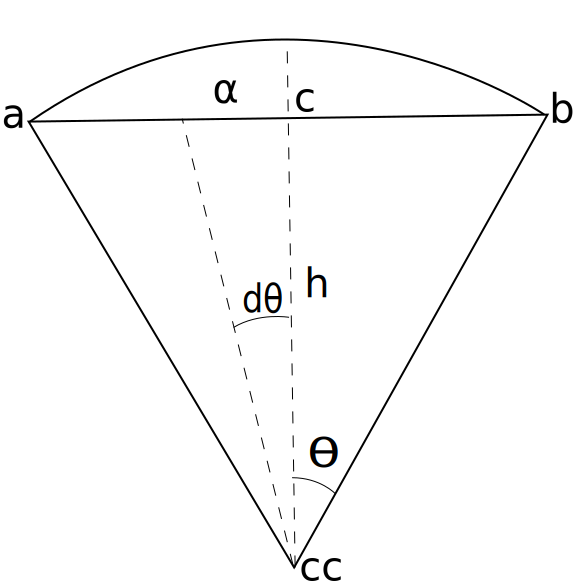
\includegraphics[width = 0.5\textwidth]{Figures/curvature.pdf}
    \caption{A sketch of the curved edge and the variables necessary to calculate the projection}
    \label{fig:curvature}
\end{figure}


\begin{itemize}
	\item initial script
	\item changes and modifications
	\item performance testing
	\item pitfalls
\end{itemize}


 
% Chapter 5

\chapter{Results} % Main chapter title

\label{results} % For referencing the chapter elsewhere, use \ref{Chapter1} 

\lhead{Chapter 6. \emph{Results and Discussion}} % This is for the header on each page - perhaps a shortened title

%----------------------------------------------------------------------------------------

\section{Drag and lift on a cylinder}
The effect of the algorithm explained in Chapter~\ref{xyzarc} is
illustrated by solving a laminar flow test problem. 
The solution is compared with previously benchmark computations performed by a number of 
contributors~\cite{benchmark}. 

The results can be found in 
table~\ref{tab:testcase}. As the results clearly show the treatment of the geometry is 
crucial, both coefficients are computed with significantly better accuracy. 
%
\begin{table}
\centering
\begin{tabular}{l l c c c c}
		\toprule
		\# of Cells & Software & $c_D$ & $c_L$ & \%\textbf{Err} $c_D$ &\%\textbf{Err} $c_L$ \\ \midrule 
		2070 & Nek5000 (mid) & 6.18349 & 0.008939 & 0.030 & 4.19 \\ 
		2070 & Nek5000 (arc) & 6.18498 & 0.009413 & 0.006 & 0.13 \\
		3145728 & CFX 		 & 6.18287 & 0.009387 & 0.04 &0.15 \\
		3145728 & OF	     & 6.18931 & 0.00973 & 0.06 &3.5 \\
		3145728 & FEATFLOW   & 6.18465 & 0.009397 & 0.01 &0.05 \\
		\bottomrule	
	\end{tabular}
	\caption{Results for the drag and lift coefficients with reference values 
	$c_D = 6.18533$ and $c_L = 0.009401$.}
\label{tab:testcase}
\end{table}
%
The polynomial degree used in the calculations with Nek5000 was chosen as $p = 11 $ 
in all directions. The explicit number of cells is therefore $2070\cdot11^{3} = 2755170$,
approximately $88\%$ of the number of cells used for the benchmark simulations. Compared 
with the results from the other softwares applied in~\cite{benchmark} Nek5000 performs 
just as well or better in most cases. It should be mentioned that the division of the grid is done 
differently for Nek5000 so the comparison is not as direct as it may seem from the table.

\colorbox{yellow}{add more info about the mesh for this case??}

\subsection{Parameter adjustments in Nek5000}
As discussed in chapter~\ref{nek} there are many adjustments available in Nek. 
In order to enlighten the actual effect on the results, several different settings have 
been investigated and the results are presented. All simulations are performed as 
transient flows and the data collected in table~\ref{tab:perf} are gathered when the 
flow has reached a steady state solution. 

\colorbox{green}{Perform the different tests and show the difference.}

\begin{table}[h]
    \centering
    \begin{tabular}{c | c c c c | c c | c c c}

         & \multicolumn{4}{|c|}{Settings} & \multicolumn{2}{|c|}{\% Error} & \multicolumn{3}{|c}{Data} \\\hline
         \#  & ifsplit & Dealiasing & IOFS & Filter & $c_D$ & $c_L$ & DT & CFL & T/Tstep \\ \hline 
         1 & F & F & F & F & 1.0 & 2.3 & 1e-04 & 2.03 & 2.1e-02 \\
         2 & T & T & F & F & 1.0 & 2.3 & 1e-04 & 2.03 & 2.1e-02 \\
         3 & F & T & F & T & 1.0 & 2.3 & 1e-04 & 2.03 & 2.1e-02 \\
         4 & F & T & T & T & 1.0 & 2.3 & 1e-04 & 2.03 & 2.1e-02 \\
    \end{tabular}
    \caption{Performance data for different settings in Nek5000}
    \label{tab:perf}
\end{table}
%----------------------------------------------------------------------------------------
\section{Gas dispersion in a simplified urban area} 
This case is a part of a larger project designed to evaluate different solvers 
ability to perform simulations of gas dispersion. An initial attempt to simulate the 
dispersion of gas was performed in Nek5000 with fairly coarse element sizes, but without
any subgrid-scale model. Only applying filtering on the last 3 nodes made the solution 
sufficiently stable and the results can be seen in figures~\ref{fig:cHfilter} and~\ref{fig:cHfilter}.
%
\begin{figure}[h]
	\centering
	\includegraphics[width=0.6\textwidth]{Figures/plume.png}
	\caption{A average iso-surface of the released gas at $C=0.03$ 
    after 30 seconds of sampling.}
	\label{fig:plume}
\end{figure}
%
%
\begin{figure}[h]
	\centering
	\includegraphics[width=0.8\textwidth]{Figures/NekcH.pdf}
	\caption{Time-averaged concentration with a sample time of $18.00$ s at $z/H = 0.025$ plotted horizontally and scaled 
	with the free-stream velocity and emission rate. Compared against wind tunnel data.
Two dashed lines on either side of the centerline represent the canyon.}
	\label{fig:cHfilter}
\end{figure}
%
Discuss the plot... 

%
\begin{figure}[h]
	\centerline{\includegraphics[width=1.2\textwidth]{Figures/vel_field.png}}
	\caption{velocity field for $z= 0.02$m, around the source and the cubes.}
	\label{fig:vel_field}
\end{figure}
%

\colorbox{green}{redo these simulation in case they were started to early.}
%
\begin{figure}[h]
	\centering
	\includegraphics[width=0.8\textwidth]{Figures/NekcV.pdf}
	\caption{Time-averaged concentration with a sample time of $18.00$ s at $y = 0$ plotted
    vertically and scaled 
	with the free-stream velocity and emission rate. Compared against wind tunnel data.
Two dashed lines on either side of the centerline represent the canyon.}
	\label{fig:cVfilter}
\end{figure}
%

\subsection{Dynamic Smagorinsky}
Applying a subgrid scale model to the problem should imply a more accurate result 
since the grid is not sufficiently fine to resolve the finest eddies. 
%
\begin{figure}[h]
	\centering
	\includegraphics[width=0.8\textwidth]{Figures/Nek_smag_cV.pdf}
	\caption{Time-averaged concentration with a sample time of $22.00$ s at $y = 0$ plotted
    vertically and scaled 
	with the free-stream velocity and emission rate. Compared against wind tunnel data.
Two dashed lines on either side of the centerline represent the canyon.}
	\label{fig:cVsmag}
\end{figure}
%
%
\begin{figure}[h]
	\centering
	\includegraphics[width=0.8\textwidth]{Figures/Nek_smag_cH.pdf}
	\caption{Time-averaged concentration with a sample time of $22.00$ s at $y = 0$ plotted
    vertically and scaled 
	with the free-stream velocity and emission rate. Compared against wind tunnel data.
Two dashed lines on either side of the centerline represent the canyon.}
	\label{fig:cVsmag}
\end{figure}
%
%
\begin{figure}[h]
	\centering
	\includegraphics[width=0.8\textwidth]{Figures/Nek_smag_cfluctH.pdf}
	\caption{Time-averaged concentration with a sample time of $22.00$ s at $y = 0$ plotted
    vertically and scaled 
	with the free-stream velocity and emission rate. Compared against wind tunnel data.
Two dashed lines on either side of the centerline represent the canyon.}
	\label{fig:cVsmag}
\end{figure}
%

\section{Discussion and Conclusion}
\colorbox{green}{How did Nek perform overall, user-friendly ?,correctness,speed etc.}

 
%\input{Chapters/Chapter5} 
%\input{Chapters/Chapter6} 
%\input{Chapters/Chapter7} 

%----------------------------------------------------------------------------------------
%	THESIS CONTENT - APPENDICES
%----------------------------------------------------------------------------------------

\addtocontents{toc}{\vspace{2em}} % Add a gap in the Contents, for aesthetics

\appendix % Cue to tell LaTeX that the following 'chapters' are Appendices

%% Include the appendices of the thesis as separate files from the Appendices folder
%% Uncomment the lines as you write the Appendices

% Appendix A

\chapter{Fundamental basics of numerical analysis} % Main appendix title

\label{AppendixA} % For referencing this appendix elsewhere, use \ref{AppendixA}

\lhead{Appendix A. \emph{Numerical analysis}} % This is for the header on each page - perhaps a shortened title

\section{Essential polynomials}
\begin{enumerate}
    \item Legendre polynomials
    \item Lagrange basis 
\end{enumerate}

\section{Preliminary concepts}

\begin{enumerate}
    \item coersiveness
    \item Bounded  
\end{enumerate}

\section{Lax-Milgram theorem}

Stating the theroem without proof 


% Appendix Template

\chapter{Variables and Functions in Nek5000} % Main appendix title

\label{AppendixB} % Change X to a consecutive letter; for referencing this appendix elsewhere, use \ref{AppendixX}

\lhead{Appendix B. \emph{Variables and functions in Nek}} % Change X to a consecutive letter; this is for the header on each page - perhaps a shortened title

\section{Variables}

\section{Functions}

%%\input{Appendices/AppendixC}

\addtocontents{toc}{\vspace{2em}} % Add a gap in the Contents, for aesthetics

\backmatter

%----------------------------------------------------------------------------------------
%	BIBLIOGRAPHY
%----------------------------------------------------------------------------------------

\label{Bibliography}

\lhead{\emph{Bibliography}} % Change the page header to say "Bibliography"

\bibliographystyle{unsrtnat} % Use the "unsrtnat" BibTeX style for formatting the Bibliography

\bibliography{Bibliography} % The references (bibliography) information are stored in the file named "Bibliography.bib"

\end{document}  
